\vfill\null
\subsection{Exercise 26.4}

\noindent \hspace{1.2em}\textit{Find the absolute maximum value and the absolute minimum value of the following functions (Question 1 to 3):}
\begin{enumerate}
      \begin{multicols}{2}
            \item $f(x)=5-36 x+3 x^2+4 x^3$, $[-1,2]$
            \sol{}
            \begin{flalign*}
                  f'(x)                          & = 12x^2 + 6x - 36  & \\
                  12x^2 + 6x - 36                & = 0                & \\
                  2x^2 + x - 6                   & = 0                & \\
                  (2x - 3)(x + 2)                & = 0                & \\
                  x               = \dfrac{3}{2} & \text{ or } x = -2
            \end{flalign*}
            \begin{flalign*}
                  f\left(\dfrac{3}{2}\right) & = 5 - 36\left(\dfrac{3}{2}\right) + 3\left(\dfrac{3}{2}\right)^2 + 4\left(\dfrac{3}{2}\right)^3 = -\dfrac{115}{4} & \\
                  f(-1)                      & = 5 - 36(-1) + 3(-1)^2 + 4(-1)^3 = 40                                                                             & \\
                  f(2)                       & = 5 - 36(2) + 3(2)^2 + 4(2)^3 = -23
            \end{flalign*}
            $\therefore$ Absolute maximum value is $40$ and absolute minimum value is $-\dfrac{115}{4}$ in the interval $[-1,2]$.

            \item $f(x)=4 x^2\left(x^2-2\right)$, $[-1,3]$
            \sol{}
            \begin{flalign*}
                  f(x)         & = 4x^4 - 8x^2         & \\
                  f'(x)        & = 16x^3 - 16x         & \\
                  16x(x^2 - 1) & = 0                   & \\
                  x = 0        & \text{ or } x = \pm 1
            \end{flalign*}
            \begin{flalign*}
                  f(-1) & = 4(-1)^4 - 8(-1)^2 = -4 & \\
                  f(0)  & = 4(0)^4 - 8(0)^2 = 0    & \\
                  f(1)  & = 4(1)^4 - 8(1)^2 = -4   & \\
                  f(3)  & = 4(3)^4 - 8(3)^2 = 252
            \end{flalign*}
            $\therefore$ Absolute maximum value is $252$ and absolute minimum value is $-4$ in the interval $[-1,3]$.
      \end{multicols}
      \vfill\null

      \newpage
      \item $f(x)=x^5-5 x^4+5 x^3$, $[0,4]$
            \sol{}
            \begin{flalign*}
                  f'(x)              & = 5x^4 - 20x^3 + 15x^2              & \\
                  5x^2(x^2 - 4x + 3) & = 0                                 & \\
                  x^2(x - 3)(x - 1)  & = 0                                 & \\
                  x = 0              & \text{ or } x = 1 \text{ or } x = 3
            \end{flalign*}
            \begin{flalign*}
                  f(0) & = (0)^5 - 5(0)^4 + 5(0)^3 = 0   & \\
                  f(1) & = (1)^5 - 5(1)^4 + 5(1)^3 = 1   & \\
                  f(3) & = (3)^5 - 5(3)^4 + 5(3)^3 = -27 & \\
                  f(4) & = (4)^5 - 5(4)^4 + 5(4)^3 = 64
            \end{flalign*}
            $\therefore$ Absolute maximum value is $64$ and absolute minimum value is $-27$ in the interval $[0,4]$.
            \vfill\null

            \begin{multicols}{2}
                  \item A metal wire with a length of $60$cm is bent into a rectangle. Find the width
                  and the length of the rectangle so that the area of the rectangle is the
                  largest. \sol{}

                  Let the width and length of the rectangle be $x$ and $y$ respectively,
                  \begin{flalign*}
                        2x + 2y & = 60     & \\
                        y       & = 30 - x
                  \end{flalign*}
                  Let $f(x) = xy$,
                  \begin{flalign*}
                        f(x)    & = x(30 - x)    & \\
                                & = 30x - x^2    & \\
                        f'(x)   & = 30 - 2x      & \\
                        30 - 2x & = 0            & \\
                        x       & = 15           & \\
                        y       & = 30 - 15 = 15 & \\
                        f''(x)  & = -2 < 0
                  \end{flalign*}
                  $\therefore$ The width and length of the rectangle are $15$cm and $15$cm respectively for the area of the rectangle to be the largest.

                  \item A metal wire with a length of $100$cm is cut into two sections. Each section is
                  bent into a square. Find the length of these two sections of the wire so that
                  the sum of the areas of the two squares is the smallest. \sol{}

                  Let the side length of the two squares be $x$ and $y$ respectively,
                  \begin{flalign*}
                        4x + 4y & = 100    & \\
                        y       & = 25 - x
                  \end{flalign*}
                  Let $A(x) = x^2 + y^2$,
                  \begin{flalign*}
                        A(x)    & = x^2 + (25 - x)^2 & \\
                                & = 2x^2 - 50x + 625 & \\
                        A'(x)   & = 4x - 50          & \\
                        4x - 50 & = 0                & \\
                        x       & = 12.5             & \\
                        y       & = 25 - 12.5 = 12.5 & \\
                        A''(x)  & = 4 > 0
                  \end{flalign*}
                  $\therefore$ The length of the two sections of the wire are both $4(12.5) = 50$cm.
            \end{multicols}
            \vfill\null

            \newpage
      \item As shown in the diagram below, a trapezium has three sides of length $10$cm.If
            the area of the trapezium is the largest, find the length of the fourth side.
            Hence, find the maximum area of the trapezium.
            \begin{center}
                  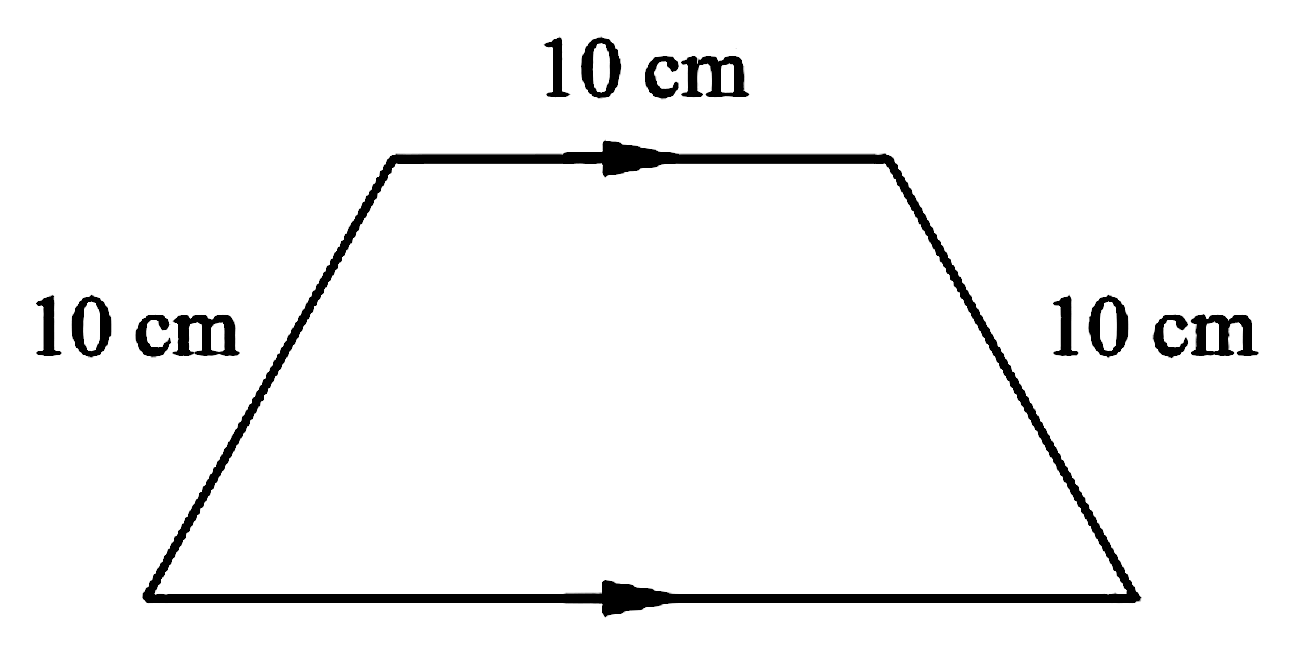
\includegraphics[scale=0.25]{assets/26-11.png}
            \end{center}
            \sol{}

            Let the length of the fourth side be $2x + 10$cm,
            \begin{flalign*}
                  h               & = \sqrt{100 - x^2}                                        & \\
                  A               & = \dfrac{1}{2}(2x + 10 + 10)\left(\sqrt{100 - x^2}\right) & \\
                                  & = (x + 10)\sqrt{100 - x^2}                                & \\
                  A'              & = \sqrt{100 - x^2} - \dfrac{x(x + 10)}{\sqrt{100 - x^2}}  & \\
                  0               & = \sqrt{100 - x^2} - \dfrac{x(x + 10)}{\sqrt{100 - x^2}}  & \\
                  0               & = 100-x^2-x^2-10x                                         & \\
                  x^2 + 5x - 50   & = 0                                                       & \\
                  (x + 10)(x - 5) & = 0                                                       & \\
                  x               & = 5 \text{ or } x = -10 \text{ (rejected)}
            \end{flalign*}
            $\therefore$ The length of the fourth side is $2(5) + 10 = 20$cm and the maximum area of the trapezium is $(5 + 10)\sqrt{100 - 5^2} = 75\sqrt{3}$cm$^2$.

      \item A right cone has a slant height of $9$cm. Find the height of the cone such that
            the volume of the cylinder is the largest. \sol{}

            Let the radius and height of the cone be $r$ and $h$ respectively,
            \begin{flalign*}
                  V     & = \dfrac{1}{3}\pi r^2h          & \\
                  r     & = \sqrt{81 - h^2}               & \\
                  V     & = \dfrac{1}{3}\pi(81 - h^2)h    & \\
                        & = 27\pi h - \dfrac{1}{3}\pi h^3 & \\
                  V'    & = 27\pi - \pi h^2               & \\
                  27\pi & = \pi h^2                       & \\
                  h     & = 3\sqrt{3} \text{cm}\ (h > 0)  & \\
                  V''   & = -2\pi h < 0
            \end{flalign*}
            $\therefore$ The height of the cone is $3\sqrt{3}$cm in order for the volume of the cone to be the largest.

            \newpage
      \item A cylinder shaped can with lid has a volume of $250\pi$cm$^3$. Find the bottom
            radius and the height of the can so that the material used is the least. \sol{}

            Let the radius and height of the can be $r$ and $h$ respectively,
            \begin{flalign*}
                  V      & = \pi r^2h                                       & \\
                  h      & = \dfrac{250}{r^2}                               & \\
                  A      & = 2\pi r^2 + 2\pi rh                             & \\
                         & = 2\pi r^2 + 2\pi r\left(\dfrac{250}{r^2}\right) & \\
                         & = 2\pi r^2 + \dfrac{500\pi}{r}                   & \\
                  A'     & = 4\pi r - \dfrac{500\pi}{r^2}                   & \\
                  4\pi r & = \dfrac{500\pi}{r^2}                            & \\
                  r^3    & = 125                                            & \\
                  r      & = 5 \text{cm}                                    & \\
                  h      & = \dfrac{250}{5^2} = 10 \text{cm}                & \\
                  A''    & = 12\pi r + \dfrac{1000\pi}{r^3} > 0
            \end{flalign*}
            $\therefore$ The bottom radius and the height of the can are $5$cm and $10$cm respectively in order for the material used to be the least.

      \item Split the number 20 into two parts such that the sum of 4 times the reciprocal
            of one part with 9 times the reciprocal of another part is the smallest. \sol{}

            Let the two parts be $x$ and $y$ respectively,
            \begin{flalign*}
                  x + y = 20 \implies y = 20 - x &
            \end{flalign*}
            Let $S = \dfrac{4}{x} + \dfrac{9}{y}$,
            \begin{flalign*}
                  S(x)               & = \dfrac{4}{x} + \dfrac{9}{20 - x}        & \\
                  S'(x)              & = -\dfrac{4}{x^2} + \dfrac{9}{(20 - x)^2} & \\
                  0                  & = -\dfrac{4}{x^2} + \dfrac{9}{(20 - x)^2} & \\
                  \dfrac{4}{x^2}     & = \dfrac{9}{(20 - x)^2}                   & \\
                  4(20 - x)^2        & = 9x^2                                    & \\
                  4x^2 - 160x + 1600 & = 9x^2                                    & \\
                  x^2 + 32x - 320    & = 0                                       & \\
                  (x + 40)(x - 8)    & = 0                                       & \\
                  x = 8              & \text{ or } x = -40 \text{ (rejected)}
            \end{flalign*}
            $\therefore$ The two parts are $8$ and $12$ respectively in order for the sum to be the smallest.

            \begin{multicols}{2}
                  \item A metal wire with a length of $150$cm is split into two sections, and they are
                  bent into a square and a circle respectively. Find the length of these two
                  sections such that the sum of the area of the square and the circle is the
                  smallest. \sol{}

                  Let the side length and the radius of the square and the circle be $s$ and $r$
                  respectively,
                  \begin{flalign*}
                        4s + 2\pi r & = 150                                            & \\
                        r           & = \dfrac{75 - 2s}{\pi}                           & \\
                        A           & = s^2 + \pi r^2                                  & \\
                                    & = s^2 + \pi\left(\dfrac{75 - 2s}{\pi}\right)^2   & \\
                                    & = s^2 + \dfrac{(75 - 2s)^2}{\pi}                 & \\
                        A'          & = 2s - \dfrac{4(75 - 2s)}{\pi}                   & \\
                        2s          & = \dfrac{4(75 - 2s)}{\pi}                        & \\
                        2\pi s      & = 4(75 - 2s)                                     & \\
                        2\pi s      & = 300 - 8s                                       & \\
                        2(\pi + 4)s & = 300                                            & \\
                        s           & = \dfrac{150}{\pi + 4}                           & \\
                        r           & = \dfrac{75}{\pi} - \dfrac{2(150)}{\pi(\pi + 4)} & \\
                                    & = \dfrac{75(\pi + 4) - 300}{\pi(\pi + 4)}        & \\
                                    & = \dfrac{75\pi + 300 - 300}{\pi(\pi + 4)}        & \\
                                    & = \dfrac{75\pi}{\pi(\pi + 4)}                    & \\
                                    & = \dfrac{75}{\pi + 4}
                  \end{flalign*}
                  $\therefore$ The length of the two sections are $4\left(\dfrac{150}{\pi + 4}\right) = \dfrac{600}{\pi + 4}$cm and $2\pi\left(\dfrac{75}{\pi + 4}\right) = \dfrac{150\pi}{\pi + 4}$cm respectively in order for the sum of the area to be the smallest.

                  \item A window is formed by a rectangle and a semicircle. The perimeter of the entire
                  window is 300cm. If the area of the window is the largest, find the radius of
                  the semicircle. Hence, find the maximum area of the window. \sol{}

                  Let the length of the rectangle and the radius of the semicircle be $x$cm and
                  $r$cm respectively,
                  \begin{flalign*}
                        \pi r + 2x + 2r & = 300                                                                                         & \\
                        x               & = \dfrac{300 - \pi r - 2r}{2}                                                                 & \\
                        A               & = \dfrac{1}{2}\pi r^2 + 2xr                                                                   & \\
                                        & = \dfrac{1}{2}\pi r^2 + 2r\left(\dfrac{300 - \pi r - 2r}{2}\right)                            & \\
                                        & = \dfrac{1}{2}\pi r^2 + (300 - \pi r - 2r)r                                                   & \\
                                        & = \dfrac{1}{2}\pi r^2 + 300r - \pi r^2 - 2r^2                                                 & \\
                                        & = \left(-\dfrac{1}{2}\pi - 2\right)r^2 + 300r                                                 & \\
                        A'              & = (-\pi - 4)r + 300                                                                           & \\
                        0               & = (-\pi - 4)r + 300                                                                           & \\
                        r               & = \dfrac{300}{\pi + 4}                                                                        & \\
                        x               & = 150 - \dfrac{1}{2}\pi\left(\dfrac{300}{\pi + 4}\right) - 2\left(\dfrac{300}{\pi + 4}\right) & \\
                                        & = 150 - \dfrac{150\pi}{\pi + 4} - \dfrac{600}{\pi + 4}                                        & \\
                                        & = \dfrac{150(\pi + 4) - 150\pi - 600}{\pi + 4}                                                & \\
                                        & = \dfrac{150\pi + 600 - 150\pi - 600}{\pi + 4}                                                & \\
                                        & = 0                                                                                           & \\
                        A''             & = -\pi - 4 < 0                                                                                & \\
                        A               & = \dfrac{1}{2}\pi\left(\dfrac{300}{\pi + 4}\right)^2 + 2(0)\left(\dfrac{300}{\pi + 4}\right)  & \\
                                        & = \dfrac{45000}{\pi + 4}\text{cm}^2
                  \end{flalign*}
                  $\therefore$ The radius of the semicircle is $\dfrac{300}{\pi + 4}$cm and the maximum area of the window is $\dfrac{45000}{\pi + 4}\text{cm}^2$.
            \end{multicols}

            \newpage
      \item In the diagram below, $PQRS$ is a rectangle, the coordinates of $P$ and $Q$ are
            $(-k, 0)$ and $(k, 0)$ respectively, where $k > 0$, and the two points $R$ and
            $S$ are on the curve $y = 3- \dfrac{1}{2}x^2$. Find the value of $k$ such that
            the area of the rectangle is the largest.
            \begin{center}
                  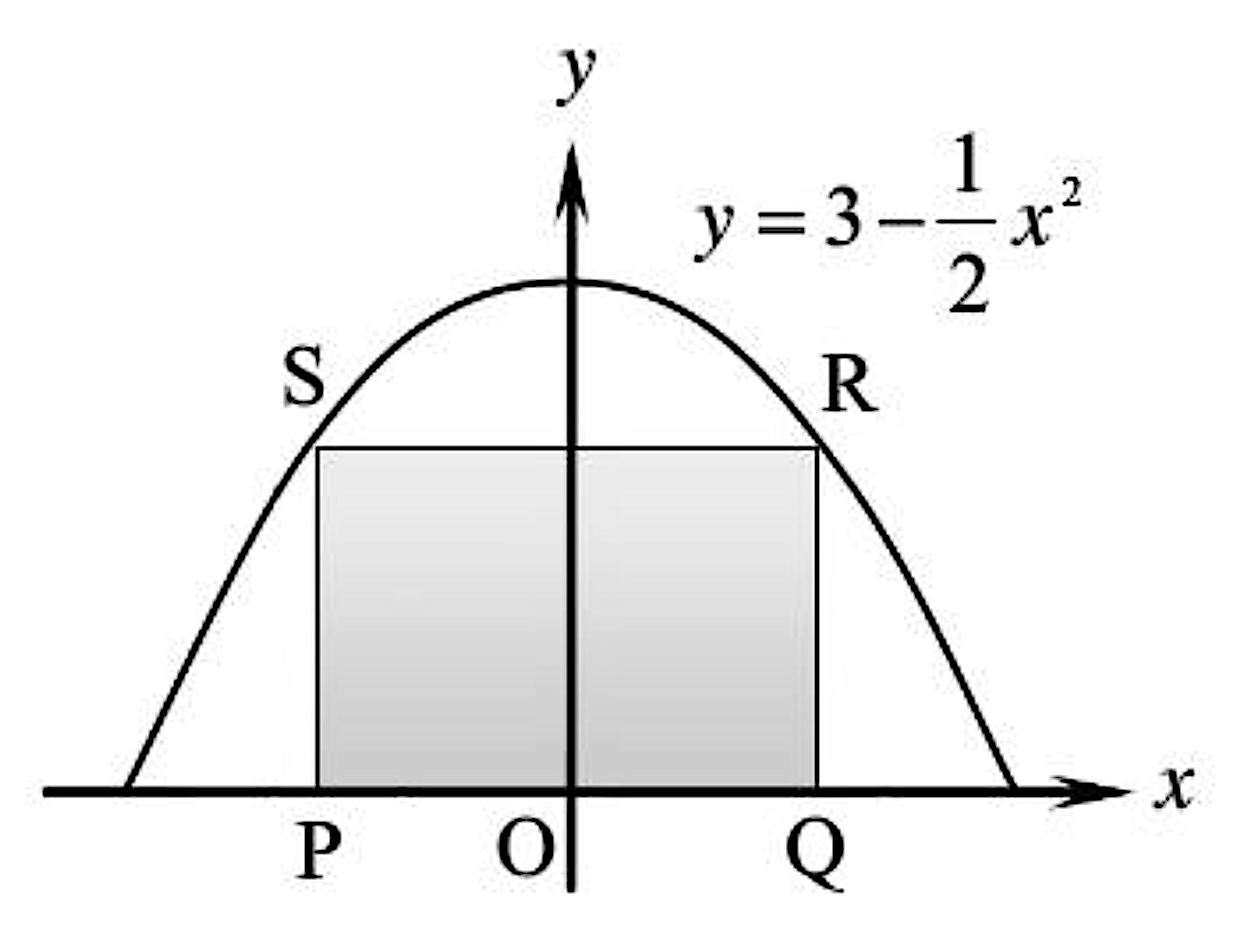
\includegraphics[scale=0.25]{assets/26-9.png}
            \end{center}
            \sol{}
            \begin{flalign*}
                  A    & = 2k\left(3 - \dfrac{1}{2}k^2\right) & \\
                       & = 6k - k^3                           & \\
                  A'   & = 6 - 3k^2                           & \\
                  0    & = 6 - 3k^2                           & \\
                  3k^2 & = 6                                  & \\
                  k^2  & = 2                                  & \\
                  k    & = \sqrt{2} \text{ (k > 0)}           & \\
                  A''  & = -6k < 0
            \end{flalign*}
            $\therefore$ The value of $k$ is $\sqrt{2}$ in order for the area of the rectangle to be the largest.

\end{enumerate}